\documentclass[11pt,
compress,
%% handout, 
%% dvips,
%% trans
]{beamer}
%% Try the class options [notes], [notes=only], [trans], [handout],
%% [red], [compress], [draft], [class=article] and see what happens!

\usepackage{bm}
\usepackage{booktabs}
\usepackage[scale=2]{ccicons}
%\usepackage{minted}
\usepackage{amsmath,amsthm,amssymb,amsfonts}
\newcommand*{\TakeFourierOrnament}[1]{{%
		\fontencoding{U}\fontfamily{futs}\selectfont\char#1}}
\newcommand*{\danger}{\TakeFourierOrnament{66}}
\usepackage[export]{adjustbox}
%\usepgfplotslibrary{dateplot}
\usepackage{wrapfig}
\usepackage{ragged2e}
\usepackage{xcolor}
\newcommand{\red}{\color{red}}
\newcommand{\mb}{\color{blue}}
\newcommand{\blue}{\color{blue}}
\newcommand{\orange}{\color{orange}}
\newcommand{\green}{\color{green}}
\usepackage{multirow}
\usepackage{tabularx}
\usepackage{transparent}
\usepackage{graphicx}
\usepackage{caption}
\newcommand{\mnb}{\color{violet}}
\newcommand{\emer}{\color{Emerald}}
\newcommand{\fogr}{\color{ForestGreen}}
\newcommand{\redor}{\color{RedOrange}}
\newcommand{\ceru}{\color{Cerulean}}
\newcommand{\yelor}{\color{black}}
\newcommand{\ored}{\color{olive}}

\newcommand{\ubar}[1]{\text{\b{$#1$}}}

\usepackage{caption}
\usepackage{subcaption}
%\lstset{language=R,
	%	basicstyle=\scriptsize\ttfamily,
	%	stringstyle=\color{black},
	%	otherkeywords={0,1,2,3,4,5,6,7,8,9},
	%	morekeywords={TRUE,FALSE},
	%	deletekeywords={data,frame,length,as,character},
	%	keywordstyle=\color{black},
	%	commentstyle=\color{blue},
	%	escapechar={?}, 
	%}
\usepackage[utf8]{inputenc}
\usepackage[english]{babel}
\usepackage{hyperref}
\usepackage{amsmath,amsthm,amssymb,pgf}
\usepackage{comment,multicol}
%\usepackage{color}
\usepackage{rotating, listings}
\usepackage{tikz}
\usepackage{booktabs}

%% If we deo not want e``(a) Text'' but ``Text'' in subfigures.
%\usepackage{subfigure}
%\renewcommand{\thesubfigure}{\null}

%% Set custom font (Source Sans Pro)


%%\usetheme{Madrid}
\usetheme{CambridgeUS}
%%\usecolortheme{default}
\usecolortheme{dolphin}


%% KAUST saturated shades
%% Purple , R 109 G 36 B 99 , HEX# 6D2463
\definecolor{kaustpurplesaturatedshade}{RGB}{109,36,99}
%% Blue , R 0 G 59 B 117 , HEX# 003B75
\definecolor{kaustbluesaturatedshade}{RGB}{0,59,117}
%% Turquoises , R 0 G 76 B 89 , HEX# 004C59
\definecolor{kaustturquoisessaturatedshade}{RGB}{0,76,89}
%% Greens , R 89 G 84 B 3 , HEX# 595403
\definecolor{kaustgreenssaturatedshade}{RGB}{89,84,3}
%% Yellow , R 100 G 60 B 0 , HEX# 643C00
\definecolor{kaustyellowsaturatedshade}{RGB}{100,60,0}
%% Orange , R 128 G 73 B 0 , HEX# 804900
\definecolor{kaustorangesaturatedshade}{RGB}{128,73,0}

%% KAUST Gray , R 181 G 171 B 161 , HEX# B5ABA1
\definecolor{kaustgrayfullcolor}{RGB}{181,171,161}

%% User custom KAUST color scheme
\setbeamercolor*{structure}{bg=kaustgrayfullcolor!20,fg=kaustbluesaturatedshade}
%% \setbeamercolor*{palette primary}{use=structure,fg=white,bg=structure.fg}
%% \setbeamercolor*{palette primary}{use=structure,fg=white,bg=structure.fg}
%% \setbeamercolor*{palette secondary}{use=structure,fg=white,bg=structure.fg!75}
%% \setbeamercolor*{palette tertiary}{use=structure,fg=white,bg=structure.fg!50!black}
%% \setbeamercolor*{palette quaternary}{fg=white,bg=black}
%% \setbeamercolor{section in toc}{fg=black,bg=white}
%% \setbeamercolor{alerted text}{use=structure,fg=structure.fg!50!black!80!black}
%% \setbeamercolor{titlelike}{parent=palette primary,fg=structure.fg!50!black}
%% \setbeamercolor{frametitle}{bg=gray!10!white,fg=PineGreen}
%% \setbeamercolor*{titlelike}{parent=palette primary}


%% %% set logo, default position bottom right corner
%% \logo{\includegraphics[height=0.75cm]{./figures/KAUST-logo-seed.pdf}}
%% add logo to frame title, position using tikz
\addtobeamertemplate{frametitle}{}{%
    \begin{tikzpicture}[remember picture,overlay]
        \node[anchor=north east,yshift=-9pt] at (current page.north
        east)%%
        {
\includegraphics[height=0.75cm]{./up_logo.png}};
    \end{tikzpicture}
}
\usepackage{verbatim}
\setbeamercovered{transparent=15}

\usepackage{algorithm}
\usepackage{algorithmic}

\newcommand{\W}{\mathcal{W}}
\newcommand{\E}{\mathcal{E}}

\def\Prob{\text{Prob}}
\def\E{\text{E}}
\def\Cov{\text{Cov}}
\def\Corr{\text{Corr}}
\def\Var{\text{Var}}
\def\Prec{\text{Prec}}

\def\qedbox{\ifvmode\else\unskip\fi~\penalty10000 \hfill{\large$\blacksquare$}}
\def\Fig#1{Figure~\ref{#1}}
\def\Tab#1{Table~\ref{#1}}
\def\Sec#1{Section~\ref{#1}}
\def\Thm#1{Theorem~\ref{#1}}
\def\Def#1{Definition~\ref{#1}}
\def\Lem#1{Lemma~\ref{#1}}
\def\Alg#1{Algorithm~\ref{#1}}
\def\Ex#1{Example~\ref{#1}}
\def\Cor#1{Corollary~\ref{#1}}
\def\eref#1{(\ref{#1})}
\def\miscinfo#1#2{{\footnotesize\indent\textsc{#1: }\ignorespaces #2}}
\def\R{\mathbb{R}}
\def\mm#1{\ensuremath{\boldsymbol{#1}}} %% version: amsmath
\def\mv#1{\ensuremath{\boldsymbol{#1}}} %% version: amsmath
\def\logit{\text{logit}}


\title[Non-Linear Joint Models for Clinical Trials]{
    Non-Linear Joint Models for Clinical Trials}

\author[Sable Walters-Somers]{Sable Walters-Somers\\
	\tiny{Department of Statistics July Honours Presentation\\
University of Pretoria\\
\vspace{2cm}}
   }

\date[24 July 2026]{}

\usepackage{listings}
\lstset{language=C}
\let\MyIncludeSourceFontSize\footnotesize
\let\MyIncludeFontSize\small
\def\MyIncludeSource#1{\lstset{basicstyle=\MyIncludeSourceFontSize}\lstinputlisting{#1}%%
    \lstset{basicstyle=\MyIncludeFontSize}}

\begin{document}

{
  \usebackgroundtemplate{\texttransparent{0.5}{
\includegraphics[width=1.05\paperwidth]{./up_building3.png}}}
  \begin{frame}
    \titlepage
  \end{frame}
}


\section{Joint Models}

\begin{frame}
	\frametitle{Joint Models}
	\vspace{-0.8cm}

	A joint model simultaneously models longitudinal (time-dependent) data and Time-To-Event (TTE) data whilst accounting for censoring.\\ \ \\

	Consider an example of cancer patients undergoing a specific treatment. In this case, the longitudinal data could be the size of a tumor and the event of interest could be whether the patient dies under that treatment. 
\end{frame}

\section{Longitudinal Models}

\begin{frame}
	\frametitle{Longitudinal Model}
	\vspace{-0,8cm}

	A longitudinal model, say $m(t, \ubar{\Psi}_i)$, allows us to model a variable of interest (often referred to as the biomarker) as time progresses. \\ \ \\

	In our example, modeling how a patients tumor changes in size allows predictions to be made regarding patient outcomes so that necessary decisions can be made in time. \\ \ \\

	Different patients will, of course, exhibit differences in how their tumors progress and how they respond to any treatments. Thus, the longitudinal model is typically a \bm{{\mb mixed-effect model}}, utilizing the fixed and random effects of patient $i$ ($\ubar{\Psi}_i$) to account for within-patient correlation and allowing for the modeling of multiple patients.
\end{frame}

\section{Survival Model}

\begin{frame}
	\frametitle{Survival Model}
	\vspace{-0.8cm}

	TTE data is modeled through a survival model. This is done by determining the relevant \bm{{\mb hazard function}} $h_i(t)$, defined as the risk of a patient experiencing the event of interest at a specific time. i.e. 

$$
h_i(t) = \lim_{\Delta t \to 0} \frac{\mathrm{P}(t < T_i \le t + \Delta t \mid T_i > t)}{\Delta t}
$$
	where $T_i$ is the time of event for patient $i$.\\ \ \\

	It is within the survival model that censoring is accounted for. Censoring is defined as the case where the time of event is not observed in a patient for any reason. For example, a patient may no longer be able to participate in the study after moving or the event may simply have not occurred during the study period. \bm{{\mb In survival models, censoring is assumed random.}}
\end{frame}

\section{Why a Joint Model?}

\begin{frame}
	\frametitle{Why a Joint Model?}
	\vspace{-0.8cm}

	We expect that a patient with a large tumor to have a lower survivability. Additionally, once those with low survivability die, we expect that the remaining patients to have smaller tumors, biasing measurements. Thus, \bm{{\mb the longitudinal model and survival model both effect each other and are not independent}}. Therefore, \bm{{\mb a joint model}} that models both processes and their dependence on each other \bm{{\mb jointly}} is required.\\ \ \\

	This allows joint models to account for non-random censoring. For example, a patient may be dissatisfied with the treatment results under the study and decide to pull out to seek another treatment.\\ \ \\

	Ultimately, by making use of a joint model, one can create a more accurate model than by modeling either process alone, allowing for more accurate conclusions about the efficacy of the treatment being studied.
\end{frame}

\section{Non-Linear Joint-Models}

\begin{frame}
	\frametitle{Non-Linear Joint Models}
	\vspace{-0.8cm}

	A typical, linear joint model may be:

$$
h_i(t, \ubar{ \Psi }_i) = h_0(t) \cdot e^{\beta \cdot f(t, \ubar{\Psi}_i)\ +\ \gamma \cdot g(\ubar{\Psi}_i)}
$$

where $h_0$ is the baseline hazard function, $f(t, \ubar{\Psi}_i)$ is the indirect effects and is some function of $m(t, \ubar{\Psi}_i)$, and $g(\ubar{\Psi}_i)$ is the direct effects.\\ \ \\

However, say that instead of simply $\beta \cdot  f(t, \ubar{\Psi}_i)$, we had some \bm{{\mb non-linear}} function of $f$, such as a square root function, a spline, or a log function. This would then be a \bm{{\mb non-linear joint model}}.
\end{frame}



\begin{frame}
	\frametitle{Why a Non-Linear Joint model?}
	\vspace{-0.8cm}

\begin{wrapfigure}{r}{0.5\textwidth}
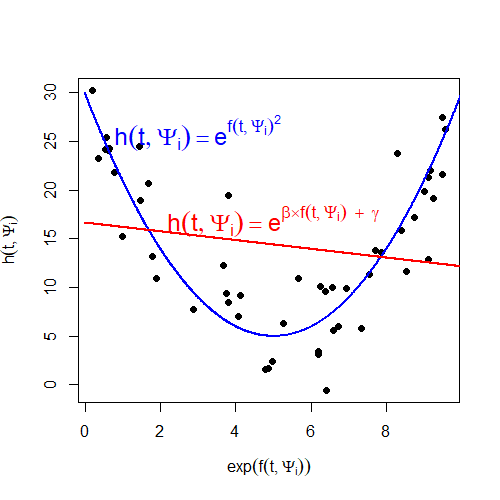
\includegraphics[width=0.5\textwidth, right]{simexample}
\end{wrapfigure}
Consider the case of type I\\ diabetes patients. These patients are at greater risk of very high and very low blood glucose levels which can both cause seizures. Thus, we expect higher risk at the extremes and minimum risk somewhere in the middle. \\ \ \\


You can see on the right a simulated example of this scenario, where the non-linear model performs very well while the linear model fails to conclude that the biomarker is even significant, attributing it a p-value of $0.23$.
\end{frame}














%\begin{frame}[fragile]
%	\frametitle{References}
%	\vspace{-1cm}
%	\small
%	\begin{itemize}
%		\item {\color{red}  Denis Rustand, Janet van Niekerk, Elias T. Krainski, H\aa vard Rue, Cécile Proust-Lima {\color{black} \textit{Fast and flexible inference for joint models of multivariate longitudinal and survival data using integrated nested Laplace approximations}}, Biostatistics, 2024; 25(2), pp.429-448, 10.1093/biostatistics/kxad019.}
		
%		\item {\color{red} Danilo  Alvares, Janet van Niekerk, Elias T. Krainski, Håvard Rue, and Denis Rustand. {\color{black} \textit{Bayesian survival analysis with INLA.}}
%			Statistics in Medicine, 2024; 1-36, 10.1002/sim.10160.}
		
%		\item {\color{red} Denis Rustand, Janet van Niekerk, Elias T. Krainski, and Håvard Rue. {\color{black} \textit{Joint Modeling of Multivariate Longitudinal and Survival Outcomes with the R package INLAjoint.}} arXiv preprint arXiv:2402.08335 (2024).}
		
%		\item {\color{red}  Denis Rustand, Janet van Niekerk, Elias T. Krainski, and Håvard Rue. {\color{black} \textit{Bayesian survival, longitudinal and joint models with INLA.}} CRC Press. 2026 (In Production).}
%	\end{itemize}
%\end{frame}


\end{document}
